%%%%% this line is 80 chars wide, please don't make longer lines %%%%%%%%%%%%%%%

\subsection{Rate modulation depth}

\begin{figure*}[ht]
	\centering
  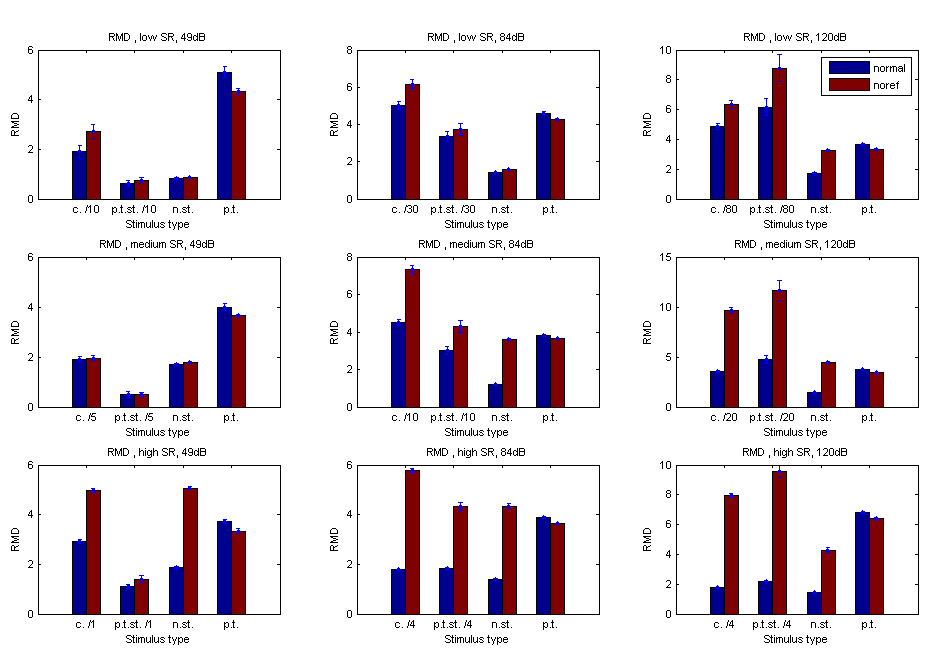
\includegraphics[width=\textwidth]{images/rmds9.png} %or jpg ?; TODO have a better one, and crop it with Paint, see if ok when printed
	\caption{RMD values for different SR fibers and intensities. Experiment labels are abbreviated 
	(c. for click, p. t. st. for pure tone step, n. st. for noise step, p. t. for pure tone).
	Some RMD results had to be scaled to fit properly in the graph and the scaling factor is written in the legend of the x-axis.
	From left to right, we have sound intensities : 49 dB, 84 dB, 120 dB,
	from top to bottom, we have fiber types : low SR, medium SR and high SR.}
	\label{fig:rmds}
\end{figure*}

For the first part of the project, an ad-hoc measure called rate 
modulation depth (RMD) was used to quantify differences between encoding 
of acoustic signal with and without an absolute refractory period (ARP) of the auditory nerve.

Four kinds of experiments where run and the average RMD was calculated 
for each of them, 
with each type of nerve fiber, and three different sound intensities : 
49 dB SPL, 84 dB SPL and 120 dB SPL (49 dB : average home, rainfall; 84 dB : busy road; 120 dB : threshold of discomfort, possible hearing loss) 
% TODO
%http://www.sengpielaudio.com/TableOfSoundPressureLevels.htm; citate ?
%http://noiselimiters.co.uk/buy/noise-levels-what-is-noise.php
to have an overall view of the effects.
For each virtual experiment, the bin size was 0.01 ms, the characteristic frequency was 1 kHz, 
there was no damage on IHC or OHC, and we told the model to use the built-in approximations 
for power-law function calculations.

The four experiments were clicks, pure tones, noise steps and pure tone steps.
The clicks were rarefaction clicks (negative pressure excursion) of 0.1 ms and sufficient time was waited between 
two of them to avoid influence from one to the other.
The two step stimuli had a period of 100 ms and in the first half of the period 
there was noise or pure tone signal, and in the second half there was 0 Pa as pressure.
The noise for the noise step was composed of random normal variables divided 
by the square root of the bin size (gaussian white noise).
The pure tone of the pure tone step was of 10 kHz frequency.

The rate modulation depth (RMD) was defined as 

\begin{equation}\label{rmdformula1} RMD =  \frac{m - b}{b}\end{equation}
%http://www.math.uiuc.edu/~hildebr/tex/displays.html

%for pure tone steps and noise steps, and as
%
%\begin{equation}\label{rmdformula2} RMD = \frac{< m >}{< b >} - 1\end{equation}
%
for clicks and pure tone steps,
where $m$ was 
the maximum of the periodogram of the encoded sounds when converted in 2 ms bins.
The meaning of the $b$ depended on the stimulus. 
For the clicks it corresponded to the mean response to a 0 Pa pressure signal,
 with same number of repetitions than for the click stimulus. 
For the noise step, the baseline is the value of the periodogram just before the second 
half of the period, so just before the stimulus offset,
 in 10 ms bins. 
The baseline for the pure tone step was the mean of PSTH values
of a response to a pure tone of the frequency used for the stimulus (10 kHz),
after the IHC were saturated (as could be seen in the potential, 
which stays constant because it has not the time 
to be depolarized between two periods of the stimulus). 
The periodogram was computed from the same number of repetitions as for the pure tone step stimulus.
For the pure tone, the baseline was chosen as the mean of the periodogram.
For pure tones and noise steps, for each repetition the RMD was calculated and the final result is the mean, whereas
for clicks and pure tone steps $b$ and $m$ where found separately and their means where then used for the RMD calculation.
%When baselines for clicks and for pure tone step where computed, 
%we took attention to the fact that the number of repetitions of stimulus
%for the used periodogram should correspond to the one for the periodogram used for 
%calculating the maximum. 
%It gives then an equivalent RMD as if we had divided each periodogram by 
%their own number of repetitions.

\autoref{fig:rmds} displays RMD values as obtained in our virtual experiments, 
for several fiber types and sound intensities. 
Error bars for noise steps and pure tones are standard deviation of the mean of the RMDs calculated for each repetition of the stimulus. 
For clicks and pure tone step, the error bars are of value $\sigma_{< RMD >}$. To find this value, the standard deviation of the means of $m$ and $b$ were calculated and then propagated for the division with \autoref{errorprop}.

\begin{equation}\label{errorprop}\frac{\sigma_{< RMD >}}{|<RMD>|}= \sqrt{\left(\frac{\sigma_{< m >}}{< m >}\right)^2 + \left(\frac{\sigma_{< b >}}{< b >}\right)^2} \end{equation}
 
As displayed on \autoref{fig:rmds}, overall effects are these:
for clicks, pure tone steps and noise steps, the RMD without absolute refractory
period is bigger than for the normal case, and it is the opposite for pure tones.

%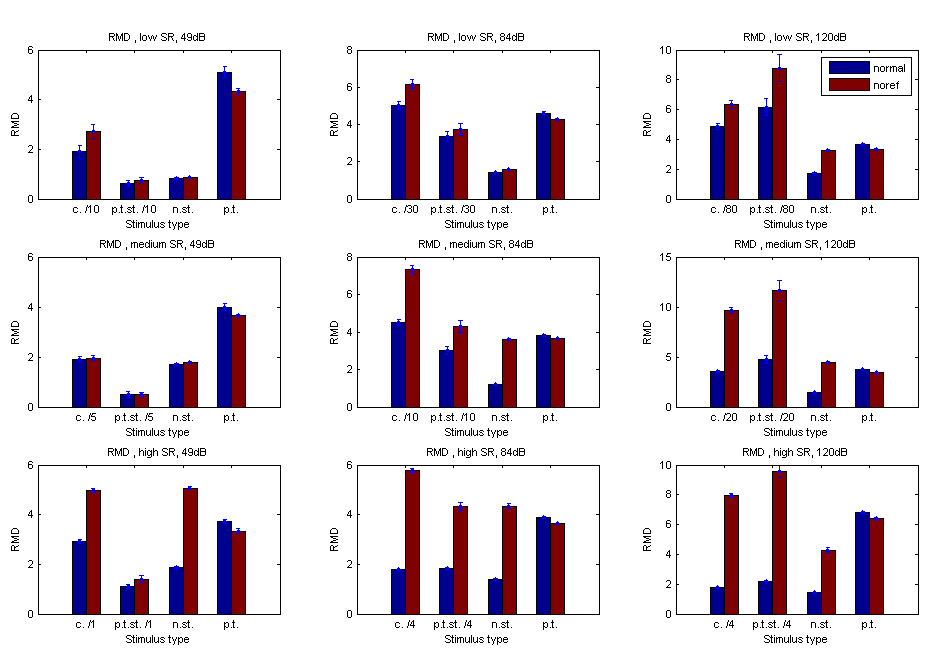
\includegraphics[width=0.45\textwidth]{images/rmds9.jpg}%put higher

We may explain the first finding because, first, we are in presence of a highly 
non-linear system and, 
secondly, the three stimuli for which the RMD without ARP is bigger, 
are stimuli with very sudden changes. 
In fact, the click can be seen as an approximation of a delta function, 
which corresponds to a broad-band stimulus. 
Also, sudden steps excite a wide range of frequencies, 
which make many non-linearities of the system contribute to the response.

%which induces a peak in the periodogram just after it, 
%and for the steps we have suddenly a signal for some time and suddenly, 
%we have no more of it, and that repeatedly, and at each of these changes, 
%we have a peak in the periodogram. 
%These peaks are then the ones which are used in the RMD computation as the maximum.
%In consequence, this RMD result can be interpreted like that : the absolute refractory period 
%seems to be able to lower the intensity of the strong response transient induced 
%when these kind of sudden changes happens.

The second finding that RMD is lower for pure tones without ARP, 
may be explained by the fact that we have less 
interactions between frequencies in the non-linear system up to the spike generator, 
in the model,
and the effects of ARP are strong enough to be seen.

\subsection{Response according to frequencies of modulated pure tones}

In \cite{Deger}, predictions are made for the absolute value (norm) and angle of the Fourier coefficients 
(harmonics 0, 1, 2 and 3) of response of stochastic point processes with refractory period,
to sinusoidal stimuli, as a function of the frequency. 
This case roughly corresponds to a tone with a high frequency carrier function, 
modulated by a low frequency oscillation. 
In fact, the inner hair cells will not be able to follow the carrier frequency 
and they will excite the nerve with a synaptic release rate dominated by the modulation.

The product of the absolute refractory period $d$ and the modulation frequency $f$,
determines the response spectrum, as shown in \autoref{fig:prednorm} (norm of Fourier coefficient) and 
\autoref{fig:predangle} (angle). Here $d$ was 80 ms. 
In the graphs, the black ligns are for harmonic 0, dark gray for 1, mid gray for 2, light gray for 3.
$\beta_k$ is the k harmonic of the output. 


%\includegraphics[page=...,viewport=llx lly urx ury,clip]{pdf-file}

\begin{figure}[h]
	\centering
	\includegraphics*[page=4,viewport=308 567 441 617]{images/Deger2010.pdf} %x, y, x, y
	\caption{Predictions for norm (\cite{Deger}  their fig. 3 (c))}
	\label{fig:prednorm}
\end{figure}

\begin{figure}[h]
	\centering
	\includegraphics*[page=4,viewport=433 567 566 619]{images/Deger2010.pdf} %x, y, x, y
	\caption{Predictions for angle (\cite{Deger} their fig. 3 (d))}
	\label{fig:predangle}
\end{figure}
%http://tex.stackexchange.com/questions/40658/extracting-image-from-pdf-to-use-in-latex-document
%pdfimages [options] <PDF-file> <image-root>, on Linux
%http://www.artofproblemsolving.com/Wiki/index.php/LaTeX:Pictures
%http://ctan.org/pkg/graphicx

\begin{figure*}[ht]
	\centering
  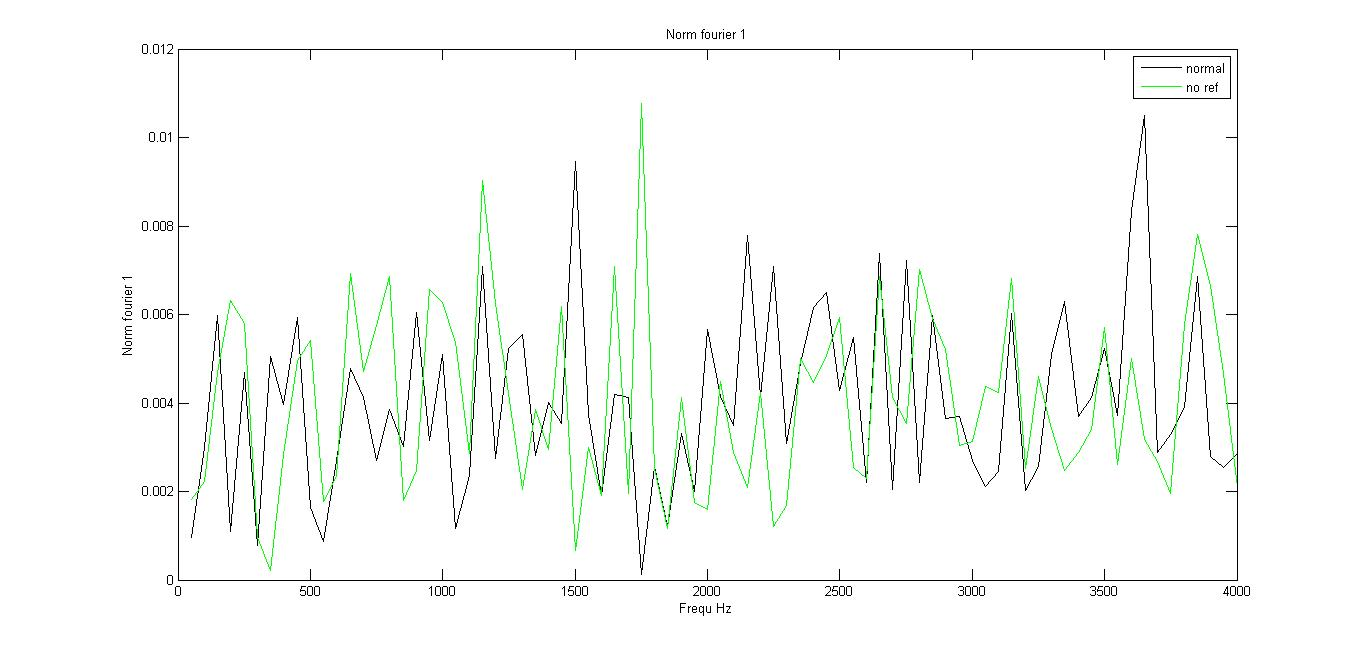
\includegraphics[width=\textwidth]{images/norm1.jpg}
	\caption{Norm of first harmonic of response to a modulated pure tone, in function of modulation frequency}
	\label{fig:norm1}
\end{figure*}

To see if the predictions are coherent with the model of the peripheral auditory 
system, experiments with modulated pure tone were run. 
The carrier frequency used was 10 kHz, the modulation frequency varied from 50 Hz to 4000 Hz
with steps of 50 Hz. We chose nerve fibers with medium SR, characteristic frequency 1 kHz 
and the stimuli were of intensity 49 dB.
The stimulis $y\left(t\right)$ were calculated like that :

\begin{equation}\label{freqstim} y\left(t\right) = A \left(1+sin \left(2 \pi t f_m \right)\right) sin \left(2 \pi t f_c \right)\end{equation} %TODO %\odot
where $A$ is the amplitude,
$f_m$ is the modulation frequency,
$f_c$ is the carrier frequency.

 
Two seconds of each stimulus were run, 
then, the second half of the PSTH was kept and its $\beta_k$ Fourier coefficients were calculated according the following formula.

\begin{equation}\label{bkformula} \beta_k = \frac{1}{T} \sum_{j= 0}^{\frac{T}{\Delta t}} e^{i \omega k j \Delta t} z \left( j \Delta t\right)\Delta t\end{equation}

where $T$ is the period (1 second here), %1sec pour tous les stimulis. expliquer ?
 $\omega$ is $\frac{2\pi}{T}$,
$\Delta t$ is the bin size (0.01ms),
$z\left(t\right)$ is the PSTH,
and $k$ is the number of the caculated harmonic.

In the model, the absolute refractory period is of 0.75 ms, so mutiples of $1/d$ are near 1333 Hz and 2666 Hz in our experiments.
Sadly, not enough data could be yet calculated to see if the results match the predictions of 
\cite{Deger}. 
As you can see in \autoref{fig:norm1}, after 10'400 repetitions, the results are too noisy to be able to conclude anything. %TODO nr rep
The graph shows the norm of the first harmonic. The other norms and angles graphs are also chaotic, so we do not show them.

%put frequ graph, even if to say : too noisy to see anything
%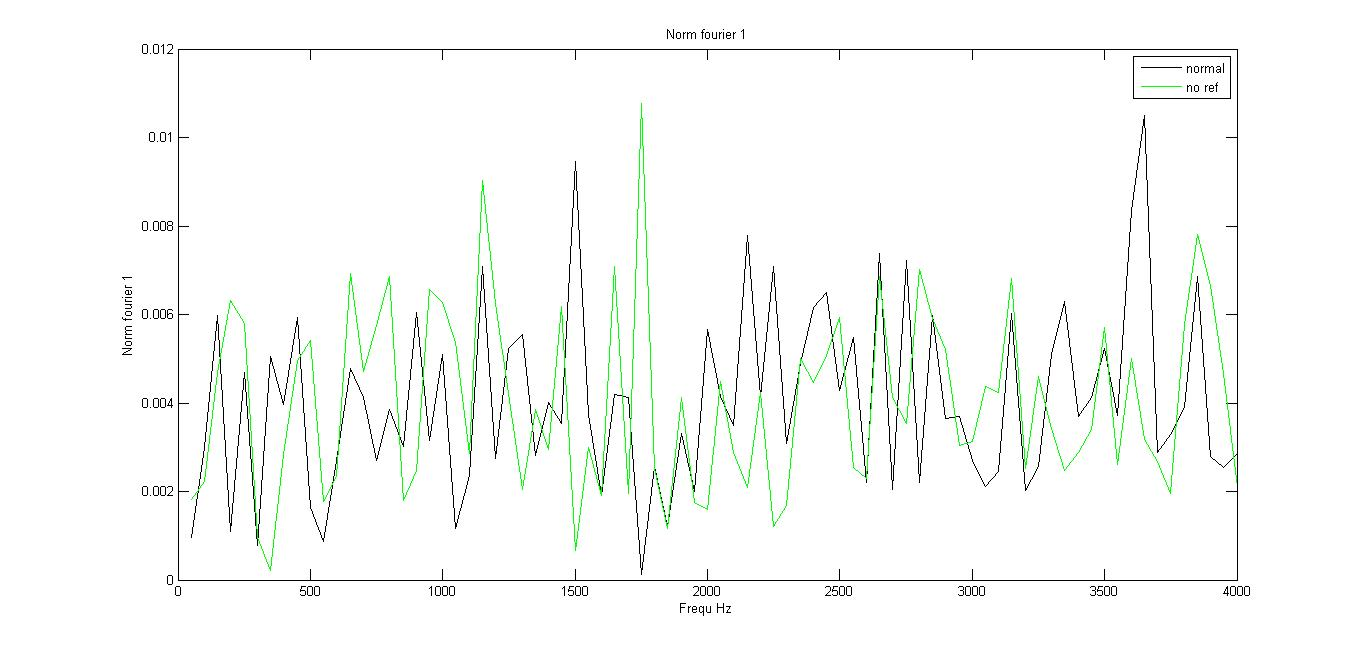
\includegraphics[width=\textwidth]{images/norm1.jpg}











 